\section{Visão}
\begin{frame}[allowframebreaks]
  \frametitle{Diferentes tipos de olhos}

  \begin{figure}[h]
  \centering
  \includegraphics[width=0.3\textwidth]{images/krilleyekils.jpg}
  \caption{Olho do Krill antártico (Euphausia superba), um pequeno crustáceo do oceano Antártico (Wikipedia).}\label{fig-krilleyekils}
  \end{figure}

  \framebreak

  \begin{itemize}
  \item Os olhos de insetos consistem em vários sensores e lentes individuais, produzindo baixa resolução, comparativamente.
  \item O camaleão pode girar os globos oculares independentemente.
  \item O cavalo possui pouca visão stereo, mas um amplo campo de visão.
  \item A acuidade e resolução visual da águia é extremamente alta.
  \item Os primatas são bem adaptados a uma visão estéreo e possuem maior sensibilidade ao vermelho que os demais animais.
  \item Os olhos do polvo evoluíram independentemente e possuem um circuito neural do lado oposto da retina, provendo boa acuidade e sensitividade a cores.
  \end{itemize}

  \framebreak 

  Nem todos animais dependem tanto da visão como nós humanos.
  \begin{itemize}
  \item Morcegos e golfinhos usam ecolocalização.
  \item Enguias geram e sentem campos elétricos.
  \item Peixes e crocodilos possuem sensores de pressão.
  \item Pássaros e abelhas possuem a capacidade de detectar a polarização da luz.
  \item Pássaros e insetos podem detectar infravermelho e ultravioleta.
  \end{itemize}

\end{frame}


\begin{frame}[allowframebreaks]
  \frametitle{Anatomia do olho humano}

  \vspace{-2ex} 
  \begin{figure}[h]
  \centering
  \includegraphics[width=0.4\textwidth]{images/schematic_diagram_of_the_human_eye_en.pdf}
  \caption{Diagrama esquemático do olho humano (Wikipedia).}\label{fig-human-eye}
  \end{figure}

  \framebreak

  \begin{figure}[h]
  \centering
  \includegraphics[width=0.7\textwidth]{images/retina.jpg}
  \caption{Camadas da retina. Cones e bastonetes (Wikipedia).}\label{fig-retina}
  \end{figure}

  \framebreak

   \begin{itemize}
   \item tamanho da abertura da lente ($5 \times 10^{-3}$ m)
   \item 160 milhões de bastonetes e cones 
   \item fóvea
   \item \hrefcolor{movimento sacádico do olho}{https://en.wikipedia.org/wiki/Saccade}
   \item ponto cego
   \item grande extensão de níveis de luminosidade, cobrindo de 9 a 10 ordem de magnitude
   \item adaptação à mudança de iluminação
   \end{itemize}
 
   \framebreak

   \begin{figure}[h]
   \centering
   \includegraphics[width=0.5\textwidth]{images/szakkad.jpg}
   \caption{Trajetória dos movimentos sacádicos do olho (Wikipedia).}\label{fig-szakkad}
   \end{figure}

   \framebreak

   Ponto cego do olho

   \vspace{8ex}
   \begin{center}
   \begin{huge}
   $\blacksquare$ \hspace{3cm} $\bigstar$
   \end{huge}
   \end{center}

   \framebreak

   \begin{figure}[h]
   \centering
   \includegraphics[width=0.6\textwidth]{images/color_sensitivity.jpg}
   \caption{Sensitividade dos cones e bastonetes (Wikipedia).}\label{fig-sensitividade}
   \end{figure}

   \framebreak

   \begin{figure}[h]
   \centering
   \includegraphics[width=0.4\textwidth]{images/photoreceptor-distribution.pdf}
   \caption{Distribuição das células fotorreceptoras no olho humano (Wikipedia).}\label{fig-photoreceptor-distribution}
   \end{figure}

\end{frame}
\note{
  ``Because of the different densities of red-, green-, and blue-sensitive cones, the overall 
sensitivity of the eye is greatest for green light and poorest for blue light.
But this sensitivity comes at a price: it is within this same range of green wavelengths 
that our ability to distinguish one color from another is poorest. 

\vspace{2ex}
Like most of the things that the eye does, the perception of color is determined in a comparative 
rather than an absolute way. It is only by comparing something to a known color reference
that we can really estimate color at all.'' \citep{russ2006}
}
\note{
``Being able to detect brightness or color is not the same thing as being able to measure it or
detect small variations in either brightness or color. While human vision functions over some
nine to ten orders of magnitude, we cannot view a single image that covers such a wide range,
nor can we detect variations of one part in $10^9$. A change in brightness of about 2 to 3\% over
a lateral distance of a few arc minutes is the limit of detectability under typical viewing conditions.

Overall, the eye can detect only about 20 to 30 shades of gray in an image, and in many cases
fewer will produce a visually satisfactory result.'' \citep{russ2006}
}
\note{
``Sensitivity to color changes at the
ends of the spectrum is much better than in the middle.
Only about a thousand different colors can be distinguished. Since
computer displays offer 256 shades of brightness for the R, G, and B phosphors, or $256^3 = 16$
million colors, we might expect that they could produce any color we can see. However, this
is not the case.'' \citep{russ2006}
}


\begin{frame}[allowframebreaks]
  \frametitle{Acuidade}

   \begin{columns}[c]
   \column{.4\textwidth}
   \begin{itemize}
   \item acuidade (resolução espacial) é normalmente especificada em unidades de ciclo por grau (ângulo)
   \item a uma distância de 50cm, 1mm representa um ângulo de pouco mais que um décimo de grau
   \item o limite superior (mais detalhes) visível do olho humano é de aproximadamente 50 ciclos por grau, ou seja,
        5 ciclos nos mesmos 1mm descritos acima, quando vistos a 50cm de distância
   \end{itemize}
   
   \column{.6\textwidth}
   \begin{figure}[h]
   \centering
   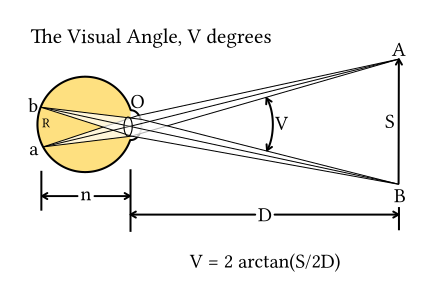
\includegraphics[width=0.9\textwidth]{images/eyeangle.pdf}
   \caption{Acuidade (Wikipedia).}\label{fig-eyeangle}
   \end{figure}
   \end{columns}
 
  \framebreak 

  \includegraphics[width=0.3\textwidth]{images/qrcode-yt-eye-res.pdf} 
  What Is The Resolution Of The Eye?\\
  \url{https://www.youtube.com/watch?v=4I5Q3UXkGd0}

  xkcd - Visual Field\\
  \url{https://xkcd.com/1080/}
\end{frame}


\begin{frame}%[allowframebreaks]
  \frametitle{Sensitividade de contraste vs. frequência espacial}

   \begin{figure}[h]
   \centering
   \includegraphics[width=0.6\textwidth]{images/contrast-sensitivity-vs-spacial-frequency.png}
   \caption{Sensitividade de contraste vs. frequência espacial (Wikipedia).}\label{fig-contrast-freq}
   \end{figure}

\end{frame}
\note{
``Enlarging images does not improve the ability to distinguish small detail, and in fact degrades
it. The common mistake made by microscopists is to work at very high magnification expecting
to see the finest details. That may be needed for details that are small in dimension, but it
will make it more difficult to see larger features that have less contrast. For the same reason,
enlarging the digitized image on the computer display does not improve, and often degrades,
the ability to see details.'' \citep{russ2006}
}

\begin{frame}[allowframebreaks]
  \frametitle{Diferenças de brilho}

   \begin{figure}[h]
   \centering
   
\includegraphics[width=0.8\textwidth]{images/bright-diff.pdf}
   \caption{Diferença de brilho.}\label{fig-bright-diff}
   \end{figure}

\end{frame}

\begin{frame}[allowframebreaks]
  \frametitle{Bandas de Mach}

   \begin{figure}[h]
   \centering
   
\includegraphics[width=0.6\textwidth]{images/mach-bands.pdf}
   \caption{Bandas de Mach.}\label{fig-mach-bands}
   \end{figure}
\end{frame}

\begin{frame}[allowframebreaks]
  \frametitle{Espiral de Fraser}

   \begin{figure}[h]
   \centering
   \includegraphics[width=0.4\textwidth]{images/Fraser_spiral.pdf}
   \caption{Espiral de Fraser (Wikipedia).}\label{fig-fraser}
   \end{figure}
\end{frame}



\begin{frame}[allowframebreaks]
  \frametitle{Ilusões ópticas}
  \centering
  \includegraphics[width=0.3\textwidth]{images/qrcode-wiki-opt-ilu.pdf}
  \url{https://en.wikipedia.org/wiki/Optical_illusion}
\end{frame}

\begin{frame}%[allowframebreaks]
  \frametitle{Leitura}
  \bibentry{russ2006}

  Capítulo 2 - \textit{Human Vision}

  \centering
  \includegraphics[width=0.3\textwidth]{images/qrcode-cap2-russ.pdf}
  \url{https://books.google.com.br/books?id=xn_MBQAAQBAJ\&lpg=PP1\&hl=pt-BR\&pg=PA83\#v=onepage\&q\&f=false}

\end{frame}

\begin{frame}%[allowframebreaks]
  \frametitle{khanacademy}
  
  \centering
  \includegraphics[width=0.3\textwidth]{images/qrcode-khanacademy-eye.pdf}
  \url{https://www.khanacademy.org/science/health-and-medicine/nervous-system-and-sensory-infor/sight-vision/v/vision-structure-of-the-eye}
\end{frame}
